\subsection{Anwendung : Streuung an harter Kugel} \marginpar{09.11.2015}
	Harte Kugel:
	\begin{align*}
	V (r) =
	\left\{
	\begin{aligned}
	\infty , r &< R, \\
	0 , r &> r
	\end{aligned}
	\right.
	\end{align*}
	$\curvearrowright$ 
	$V(r)= 0$ für $r>R \rightarrow$ Schrödingergleichung $-\frac{\hbar^2}{2m} \vec{\nabla}^2 \phi(\vec{r})
	\propto \phi(\vec{r})$
	Einsetzen in Schrödingergleichung $\Rightarrow$ Bedingungen für Koeffizienten $R_\ell(r)$:
		\begin{align*}
			R_\ell(r) &= a_\ell j_\ell (kr) + b_\ell n_\ell (kr) ,& &\text{wobei}\\
			j_\ell(\rho) &= (-\rho)^\ell \left(\frac{1}{\rho} \frac{\partial}{\partial \rho}\right)^\ell
			\frac{\sin \rho}{\rho} :& &\text{sphärische Besselfunktion}\\
			n_\ell(\rho) &= (-\rho)^\ell \left(\frac{1}{\rho} \frac{\partial}{\partial \rho}\right)^\ell
			\frac{\cos \rho}{\rho} :& &\text{sphärische Neumannfunktionen}
		\end{align*}
	$\rho \rightarrow \infty : j_\ell (\rho) \simeq \frac{1}{\rho} \sin(\rho-\ell\frac{\pi}{2})$,
	$n_\ell (\rho) \approx -\frac{1}{\rho}  \cos(\rho-\ell\frac{\pi}{2})$
	
	Einfallende Welle (2.2) besteht an $j_\ell (kr)$
	
	Auslaufende Welle $ %geschwungen
	\frac{1}{r} e^{ikr}$ (Kugelwelle)
		\begin{align*}
			h_\ell^+ (\rho) &= j_\ell (\rho) + n_\ell(\rho) \underset{r \rightarrow \infty}{\leadsto} 
			\frac{1}{i\rho} e^{i(\rho-\ell\frac{\pi}{2})} &
			&\text{(sphärische Hantelfunktion 1ter Art)} \\
			\Rightarrow \phi (\vec{r}) &= \sum_{\ell=0}^{\infty} (2 \ell +1) i^\ell
			\left[ j_\ell (kr) +\gamma_\ell h^+_\ell (kr)
			\right] P_\ell (\cos \theta)
		\end{align*}
	Randbedingung: $\phi (R, \theta, \phi)$
		\begin{align*}
			&\Rightarrow j_\ell (kR) + \gamma_\ell h_\ell^+(kR) = 0\\
			&\Rightarrow \gamma_\ell = -\frac{j_\ell(kR)}{h_\ell^+ (kR)}
		\end{align*}
	Streuamplitude:
		\begin{empheq}[box=\boxed]{align*}
			f(\theta) = \sum_{\ell = 0}^{\infty} (2 \ell +1) \frac{\gamma_\ell}{ik} P_\ell(\cos \theta)
		\end{empheq}
	Allgemein:
		\begin{align*}
			f(\theta) &= \frac{1}{k} \sum_{\ell = 0}^{\infty}
			(2 \ell + 1) \underbrace{e^{i\delta_\ell} \sin \delta_\ell}_{\mathclap{-i \gamma_\ell}}
			P_\ell (\cos \theta) \\
			\gamma_\ell &= \frac{1}{2} (e^{2i\delta_\ell} - 1)
			= -\frac{j_\ell(kR)}{j_\ell(kR)+ in_\ell (kR)}
		\end{align*}
		
		\begin{align*}
		\Rightarrow \boxed{\tan \delta_\ell = \frac{j_\ell (kR)}{n_\ell (kR)}}
		\end{align*}
		\begin{align*}
			\sigma &= \frac{4 \pi}{k^2} \sum_{\ell} (2\ell +1) 
			\frac{j_\ell^2 (kR)}{j_\ell^2 (kR)+ n_\ell^2 (kR)}
		\end{align*}
	Wobei der Bruch gleich $|\gamma_\ell|^2$
	
	Grenzfall 1: $kR \ll 1 (\gamma \gg R)$
		\begin{align*}
			j_\ell (\rho) &\underset{\rho \rightarrow 0}{\rightarrow} \frac{\rho^\ell}{(2\ell+1)!!}
			& n!! &= n(n-2) \ldots 
			& n_\ell (\rho) &\underset{\rho \rightarrow 0}{\rightarrow}
			-(2\ell + 1) !! \rho^{-(\ell +1)} \\
			\tan \delta_\ell &= -\frac{j_\ell (kR)}{n_\ell (kR)} &
			&\rightarrow - \frac{(kR)^{2\ell+1}}{(2\ell +1)!! (2\ell+1)!!} 
			& &= -\frac{(kR)^{2 \ell +1}}{(2\ell +1) [(2 \ell -1)!!]^2}
		\end{align*}
	kleine $\ell$ dominieren
		\begin{align*}
			\tan \delta_0 = - kR \approx \sin \delta \rightarrow 
			\sigma \approx \frac{\pi}{k^2} \sin^2\delta_0 + \text{höhere } \ell 
			\approx 4 \pi R^2 = 4 \sigma_{geom.}
 		\end{align*}
	Wellenlänge größer als ``Hindernis'' $\Rightarrow$ keine geom. Optik 
	\begin{figure*} [h]
		\begin{center}
			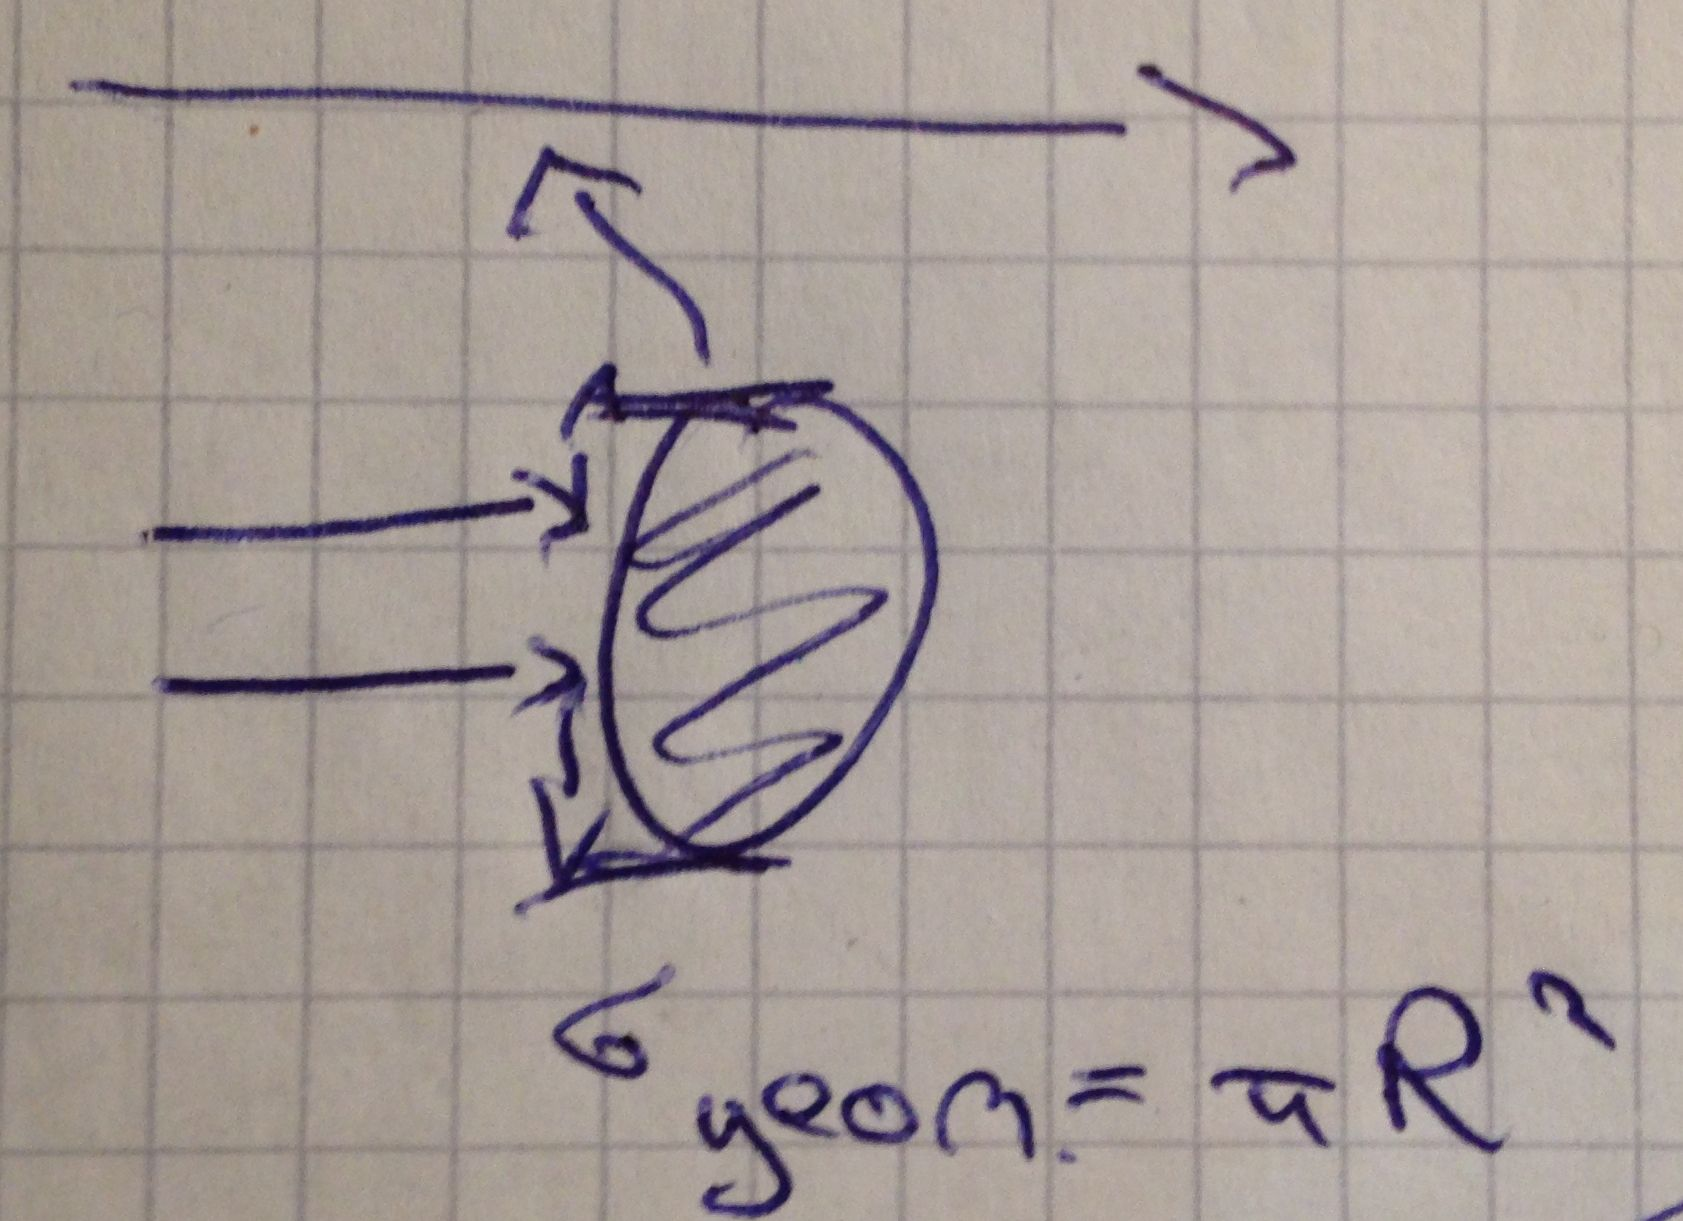
\includegraphics[width=8cm]{Annaherung_harte_Kugel1}
		\end{center}
	\end{figure*}
\FloatBarrier	
	2 Grenzfall $kR \gg1$
		\begin{align*}
			\tan \delta_\ell &\rightarrow - \frac{\sin (\rho-\ell \frac{\pi}{2})}{\cos (\rho-\ell \frac{\pi}{2})} 
			= -\tan (\rho-\ell \frac{\pi}{2}) = \tan(\ell \frac{\pi}{2} - \rho) \\
			\delta_\ell &\rightarrow \ell \frac{\pi}{2}- kR\\
			\sigma &\approx \frac{4 \pi}{k^2} \sum_{\ell =0}^{\approx int(kR)}
			(2 \ell + 1) \sin^2(\delta_\ell) 
			= \frac{4\pi}{k^2} \sum_\ell (2 \ell + 1) \sin^2(kR- \ell \frac{\pi}{2}) \\
			&\approx 2 \pi R^2 (1+ \mathscr{O} \left(\frac{1}{(kR)^{\frac{2}{3}}}\right)) 			
			\approx 2 \sigma_{geom.}
		\end{align*}
	Warum 2 $\sigma_{geom.}$? Für $\lambda \ll R$ ($k \gg \frac{1}{\ell}$) sollte klassischer Grenzfall gelten.
	\begin{figure*} [h]
		\begin{center}
			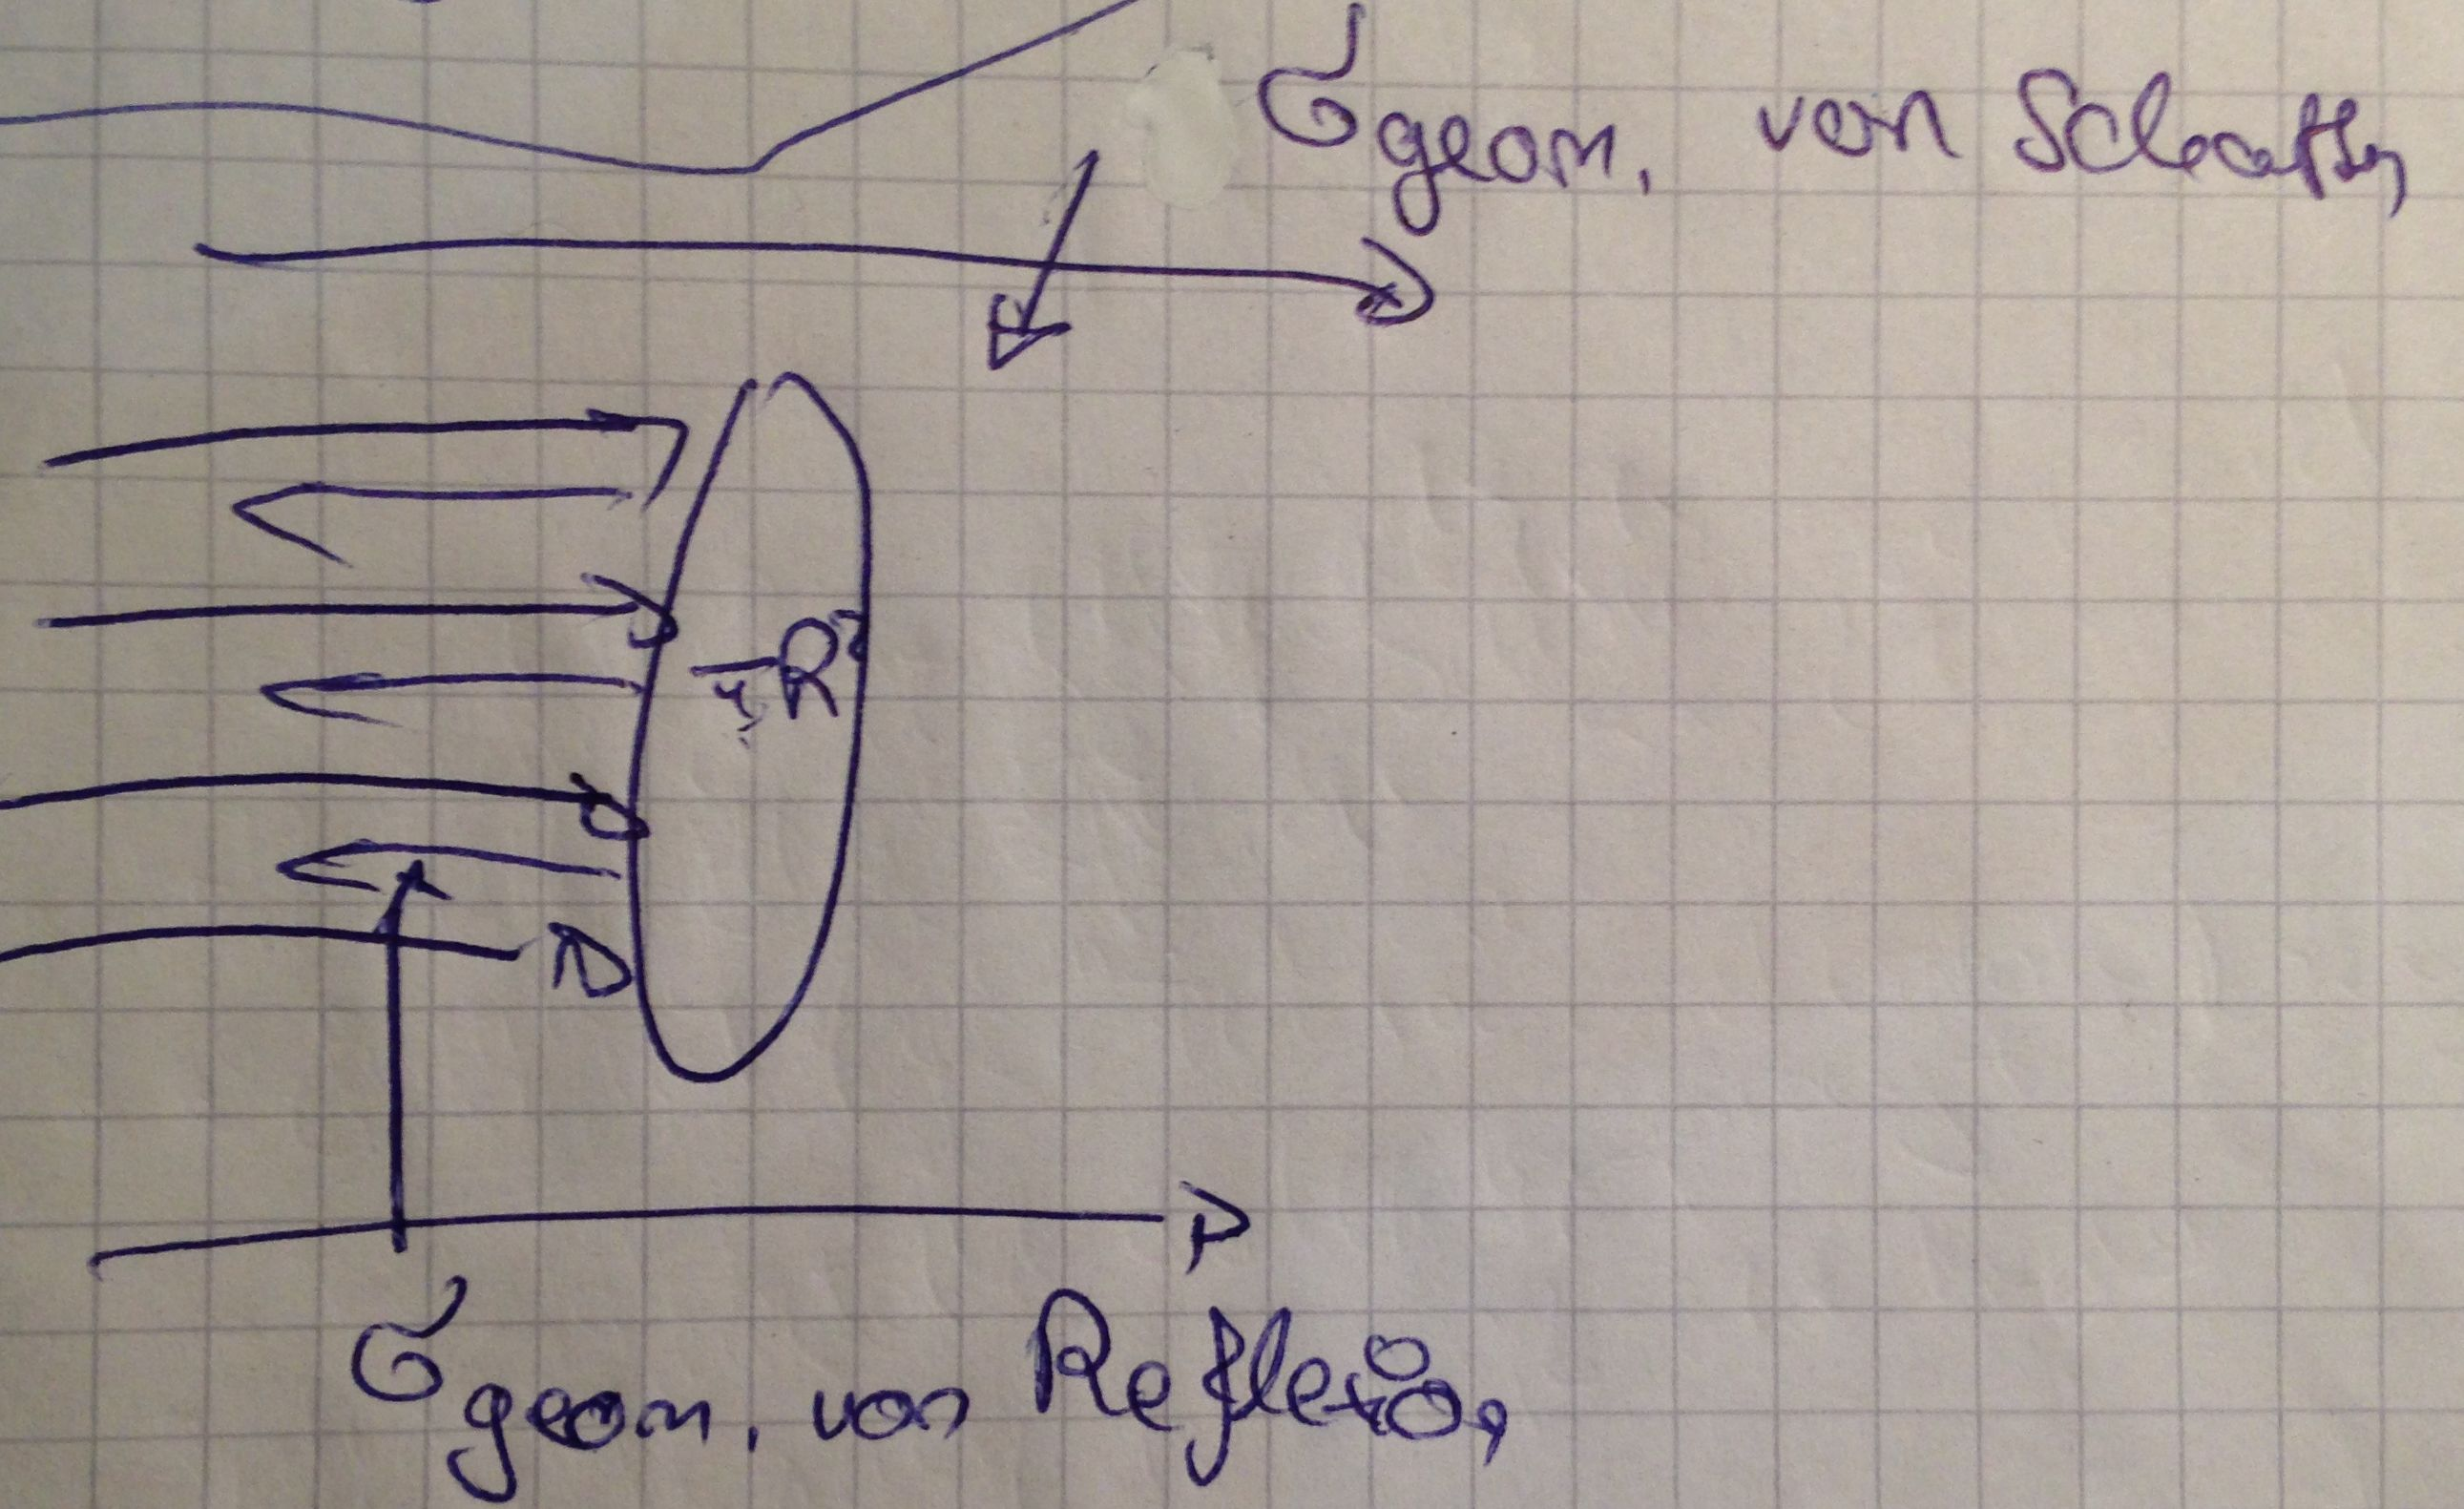
\includegraphics[width=8cm]{Annaherung_harte_Kugel2}
		\end{center}
	\end{figure*}	
	
	$\sigma$ ist so definiert, dass geometrische \textcolor{red}{Eingrpsdfjile} \marginpar{keine Ahnung was da stand}
	
	$\sigma = 2 \sigma_{geom.}$ ist